\documentclass[12pt]{article}

%% =============================================================================
% PACKAGES
%% =============================================================================

\usepackage[margin=2.54cm]{geometry}
\usepackage{graphicx}
\usepackage{booktabs}
\usepackage{subcaption}
\usepackage{pdflscape}
\usepackage{array}
\usepackage{float}
\usepackage{caption}
\usepackage{enumitem}
\usepackage{parskip}
\usepackage{microtype}
\usepackage{setspace}
\usepackage{titlesec}
\usepackage{hyperref}

\usepackage{amsmath,amssymb,amsthm}
\usepackage{mathtools}
\usepackage{nicefrac}

\usepackage{tikz}
\usetikzlibrary{positioning,arrows.meta}

\usepackage{tcolorbox}
\tcbuselibrary{skins,breakable}

\usepackage{mathptmx}

%% =============================================================================
% Section headings
%% =============================================================================

\titleformat{\section}
{\fontsize{14}{16}\selectfont\bfseries}
{\thesection}
{1em}
{}

\titleformat{\subsection}
{\fontsize{12.5}{14}\selectfont\bfseries}
{\thesubsection}
{1em}
{}

\titleformat{\subsubsection}
{\fontsize{11.5}{13}\selectfont\bfseries}
{\thesubsubsection}
{1em}
{}

%% =============================================================================
% Page layout
%% =============================================================================

\doublespacing
\setstretch{1.45}

%% =============================================================================
% Table column types
%% =============================================================================

\newcolumntype{L}[1]{>{\raggedright\arraybackslash}p{#1}}
\newcolumntype{C}[1]{>{\centering\arraybackslash}p{#1}}

%% =============================================================================
% Hyperlinks
%% =============================================================================

\hypersetup{
    colorlinks=true,
    linkcolor=black,
    citecolor=black,
    urlcolor=black,
    pdfauthor={Ethan Schroder},
    pdftitle={Bookstore Order Management System}
}

%% =============================================================================
% Boxes
%% =============================================================================

\newtcolorbox{fixbox}[1]{
  enhanced,breakable,
  colback=white,
  colframe=black,
  boxrule=0.5pt,
  arc=2pt,
  left=10pt,right=10pt,top=6pt,bottom=6pt,
  fonttitle=\bfseries,
  title={#1}
}

%% =============================================================================
% Inline code
%% =============================================================================

\newcommand{\code}[1]{\texttt{\detokenize{#1}}}

\begin{document}

%% =============================================================================
\begin{center}
\vspace*{4cm}
{\Huge \bf{Design and Implementation of a Bookstore Order Management System}}\\
\vspace{2.5cm}
{\LARGE \bf{ Ethan Schroder }}\\
\vspace*{6cm}

{\large PostgreSQL $\cdot$ Relational Database Design $\cdot$ PL/pgSQL Triggers $\cdot$ Python Application Development $\cdot$ Secure Parameterised SQL}
\end{center}

\newpage

\tableofcontents
\newpage

%% =============================================================================
\section{Introduction}
%% =============================================================================

Relational databases remain the backbone of most transactional business systems: retail ordering, insurance claims processing, and banking ledgers are all, at their core, a small number of normalised tables with carefully enforced integrity rules. What distinguishes a robust implementation from a fragile one is rarely the choice of tables, but rather where the business rules live, how consistently they are enforced, and how safely the application layer is permitted to talk to the database at all.

This report documents a small bookstore order management system built to explore exactly these questions. The system tracks a catalogue of books, a set of customers, and the orders placed between them, while automatically maintaining running sales totals, customer balances, and a full audit trail of order activity. Rather than placing this bookkeeping logic in application code, it is implemented as a set of PostgreSQL triggers and functions, so that the rules hold regardless of which client writes to the database. A Python client, built around a single class with one method per business transaction, sits on top of this schema and is used to drive both interactive use and batch transaction scripts.

\subsection{Project Overview}

The system is organised into three layers: a relational schema with declarative constraints (Section~\ref{sec:schema}), a set of database triggers and functions that implement the business rules (Section~\ref{sec:triggers}), and an object-oriented Python client that talks to the schema exclusively through parameterised queries (Section~\ref{sec:oop}). Section~\ref{sec:security} discusses the security and credential-handling decisions taken throughout. Section~\ref{sec:testing} presents the results of running the full pipeline, schema through client, against a live PostgreSQL instance. Section~\ref{sec:limitations} discusses a genuine limitation of the trigger design uncovered during that testing, and Section~\ref{sec:conclusion} concludes.

This project originated as coursework for a relational databases module and has since been reworked as a standalone, portfolio-ready piece: university-specific material and identifiers have been removed, the Python client has been rebuilt around parameterised queries and a proper class-based interface, and the whole system has been re-verified end to end against a fresh database instance rather than assumed to still work.

\newpage

%% =============================================================================
\section{Relational Schema Design}
\label{sec:schema}
%% =============================================================================

The schema has five tables. \code{book} and \code{customer} are the two core entities; \code{bookOrder} is the associative table recording which customer ordered which book, when, and in what quantity. \code{bookOrder_log} and \code{payment_log} are append-only audit tables, populated entirely by triggers rather than by direct application writes. Figure~\ref{fig:erd} shows the relationships between them.

\begin{figure}[H]
  \centering
  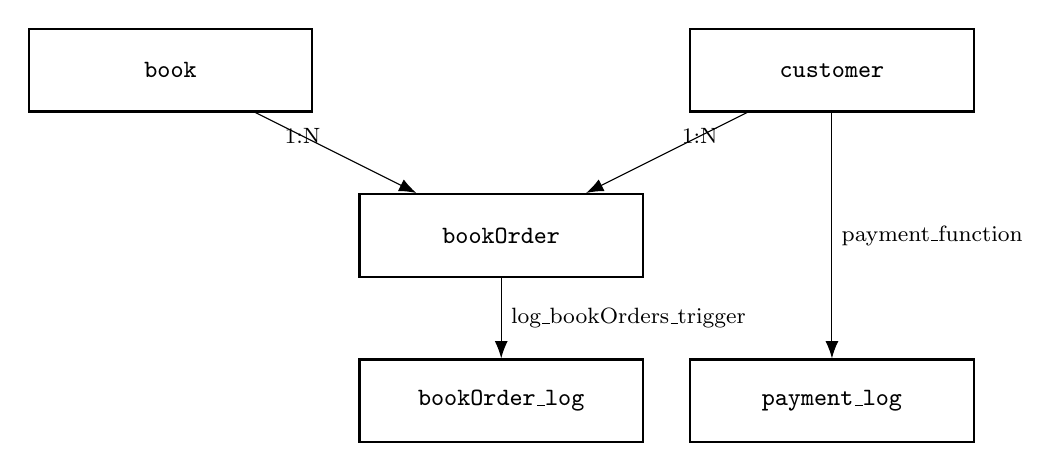
\begin{tikzpicture}[
    entity/.style={draw, thick, rectangle, minimum width=3.6cm, minimum height=1.05cm, align=center, font=\ttfamily\small},
    lbl/.style={font=\footnotesize},
    >={Latex[length=2.2mm]}
  ]
    \node[entity] (book) at (0,4.2) {book};
    \node[entity] (customer) at (8.4,4.2) {customer};
    \node[entity] (bookorder) at (4.2,2.1) {bookOrder};
    \node[entity] (bookorderlog) at (4.2,0) {bookOrder\_log};
    \node[entity] (paymentlog) at (8.4,0) {payment\_log};

    \draw[->] (book) -- (bookorder) node[lbl, midway, above left, xshift=-2pt] {1:N};
    \draw[->] (customer) -- (bookorder) node[lbl, midway, above right, xshift=2pt] {1:N};
    \draw[->] (bookorder) -- (bookorderlog) node[lbl, midway, right] {log\_bookOrders\_trigger};
    \draw[->] (customer) -- (paymentlog) node[lbl, midway, right] {payment\_function};
  \end{tikzpicture}
  \caption{Entity-relationship overview. Solid arrows from \code{book} and \code{customer} into \code{bookOrder} are foreign-key relationships; arrows into the two log tables represent trigger-populated writes rather than foreign keys.}
  \label{fig:erd}
\end{figure}

\code{bookOrder_log} and \code{payment_log} deliberately have no foreign keys back to the tables they audit. An audit trail should still be able to record that an order for a since-deleted book once existed, so these tables store the raw values rather than referencing rows that may no longer exist.

\begin{table}[H]
  \centering
  \label{tab:constraints}
  \begin{tabular}{L{2.6cm} L{5cm} L{6cm}}
    \toprule
    \textbf{Table} & \textbf{Constraint} & \textbf{Purpose} \\
    \midrule
    \code{book} & \code{bno} \code{CHECK} between 100000--999999 & keeps identifiers within a predictable, fixed-width range \\
    \code{book} & \code{category} \code{CHECK} $\in$ \{Science, Lifestyle, Arts, Leisure\} & guarantees the reporting views can group on category safely \\
    \code{customer} & \code{cno} \code{CHECK} between 100000--999999 & mirrors \code{book.bno}'s range for a consistent ID scheme \\
    \code{bookOrder} & \code{qty} \code{CHECK} $\geq 1$ & rejects zero- or negative-quantity orders at the database level \\
    \code{bookOrder} & \code{FOREIGN KEY} on \code{cno}, \code{bno} with \code{ON DELETE CASCADE} & removing a book or customer cleans up their order history rather than leaving orphan rows \\
    \bottomrule
  \end{tabular}
  \caption{Summary of integrity rules enforced declaratively at the schema level, before any trigger logic runs.}
\end{table}

\newpage

%% =============================================================================
\section{Trigger-Based Business Logic}
\label{sec:triggers}
%% =============================================================================

\subsection{Why Business Logic Lives in the Database}

An alternative design would compute \code{book.sales} and \code{customer.balance} in the Python client immediately after an order is placed. This was rejected in favour of database triggers for one reason: any client that writes directly to \code{bookOrder} (the Python client, a future web application, an ad-hoc \code{psql} session) automatically gets correct sales and balance figures, because the guarantee lives with the data rather than with any particular caller. The trade-off, discussed in Section~\ref{sec:limitations}, is that trigger semantics have to be understood precisely, since they behave differently for single-row and multi-row statements.

\begin{table}[H]
  \centering
  \small
  \begin{tabular}{L{4.8cm} L{3.3cm} L{5.4cm}}
    \toprule
    \textbf{Trigger / function} & \textbf{Fires on} & \textbf{Effect} \\
    \midrule
    \code{log_bookOrders_trigger} & any change to \code{bookOrder} & writes a row to \code{bookOrder_log} tagged \code{INSERT}/\code{UPDATE}/\code{DELETE} \\
    \code{sales_trigger} & insert into \code{bookOrder} & adds the order quantity onto \code{book.sales} \\
    \code{balance_trigger} & insert into \code{bookOrder} & adds \code{qty * price} onto the customer's \code{balance} \\
    \code{payment_function} & called explicitly & validates the customer exists, then logs a payment to \code{payment_log} \\
    \code{payment_trigger} & insert into \code{payment_log} & subtracts the payment amount from the customer's \code{balance} \\
    \bottomrule
  \end{tabular}
    \caption{Triggers and functions implementing the schema's business rules.}
    \label{tab:triggers}
\end{table}

Four reporting views sit above these tables rather than duplicating logic in the client:

\begin{itemize}[leftmargin=2em, itemsep=2pt]
\item \code{current_orders} -- orders matching a title fragment
\item \code{book_report} -- sales and value by category
\item \code{customer_report} -- books ordered per customer
\item \code{customer_bookorders} -- order history for a given customer
\end{itemize}

\newpage

\subsection{Statement-Level versus Row-Level Triggers}
\label{sec:trigger-semantics}

\code{sales_trigger} and \code{balance_trigger} are declared \code{AFTER INSERT ON bookOrder} without a \code{FOR EACH ROW} clause, making them statement-level triggers: PostgreSQL fires them once per statement, not once per affected row \cite{postgresql2026trigger}. Both trigger functions determine what changed by reading the single most recent row in \code{bookOrder_log}.

For a single-row \code{INSERT} -- exactly how \code{BookstoreClient.place_order} places every order -- this is correct: one row is inserted, one log row is written, and the statement-level trigger reads that one row back out. For a multi-row \code{INSERT INTO bookOrder VALUES (...), (...), (...)}, however, the trigger still fires only once for the whole statement, and only the last row's contribution to \code{book.sales} and \code{customer.balance} is applied. This was caught during testing (Section~\ref{sec:testing}) and is discussed further in Section~\ref{sec:limitations}.

\newpage

%% =============================================================================
\section{Object-Oriented Python Client}
\label{sec:oop}
%% =============================================================================

The Python client is built around a single guiding principle: the caller should never build a SQL string by hand, and the connection lifecycle should never be managed manually. Both are handled once, inside a single class, rather than left to whichever script happens to use the database that day.

\subsection{Class Design}

\code{BookstoreClient} owns exactly one open connection and exposes one method per business transaction: \code{insert_book}, \code{delete_book}, \code{insert_customer}, \code{delete_customer}, \code{place_order}, \code{make_payment}, and the four reporting methods corresponding to the views in Section~\ref{sec:triggers}. Table~\ref{tab:methods} summarises the interface.

\begin{table}[H]
  \centering
  \small
  \begin{tabular}{L{4.6cm} L{4.1cm} L{4.9cm}}
    \toprule
    \textbf{Method} & \textbf{Arguments} & \textbf{Returns} \\
    \midrule
    \code{insert_book} & bno, title, author, category, price & the inserted row \\
    \code{delete_book} & bno & the remaining catalogue \\
    \code{insert_customer} & cno, name, address & the inserted row \\
    \code{delete_customer} & cno & the remaining customer list \\
    \code{place_order} & cno, bno, qty & the new order line \\
    \code{make_payment} & cno, amount & a status string \\
    \code{search_orders_by_title} & title\_fragment & matching current orders \\
    \code{customer_order_history} & cno & that customer's ordered books \\
    \code{book_sales_report} & --- & sales and value by category \\
    \code{customer_summary_report} & --- & books ordered per customer \\
    \bottomrule
  \end{tabular}
    \caption{Public methods of \code{BookstoreClient}.}
    \label{tab:methods}
\end{table}

\newpage

The class supports the context manager protocol, so a connection is always closed even if an exception is raised partway through a session:

\begin{fixbox}{}
\texttt{with BookstoreClient() as db:}\\
\texttt{\ \ db.place\_order(cno=900001, bno=234567, qty=2)}\\
\texttt{\ \ print(db.book\_sales\_report())}
\end{fixbox}

\subsection{Design Principles}

\begin{itemize}[leftmargin=2em, itemsep=4pt]

  \item \textbf{Encapsulation.} Connection parameters are resolved once at construction, either from explicit arguments or from environment variables, and are never touched again. No other part of the codebase constructs a connection string.

  \item \textbf{Single responsibility.} Each method implements exactly one business transaction and returns exactly one result. \code{place_order} inserts an order line and nothing else; it does not update sales or balance figures directly, since that responsibility belongs to the triggers described in Section~\ref{sec:triggers}.

  \item \textbf{Consistent interface.} Every write method follows the same shape: set the search path, execute one parameterised statement, and return the resulting rows as a pandas \code{DataFrame}. A caller does not need to remember a different calling convention for inserts versus deletes versus reports.

  \item \textbf{Command dispatch over branching.} \code{TransactionRunner}, which drives batches of commands from a script file, maps each single-letter command code to a bound handler method through a dictionary rather than a long \code{if}/\code{elif} chain, making it straightforward to add a new command without touching existing branches.

\end{itemize}

\newpage

%% =============================================================================
\section{Security and Data Integrity}
\label{sec:security}
%% =============================================================================

\subsection{Parameterised Queries}

Every query issued by \code{BookstoreClient} is parameterised: values are passed alongside the query text and substituted by the database driver, rather than interpolated into a string beforehand. This is the standard defence against SQL injection recommended by both the Python Database API specification \cite{lemburg1999pep249} and OWASP's guidance on the subject \cite{owasp2026sqli}. Concretely, every method in \code{BookstoreClient} follows the pattern

\begin{fixbox}{}
\texttt{cur.execute(}\\
\texttt{\ \ "INSERT INTO book (...) VALUES (\%s, \%s, ...);",}\\
\texttt{\ \ (bno, title, ...)}\\
\texttt{)}
\end{fixbox}

rather than building the statement with Python string formatting. The distinction matters in practice, not only in principle: an earlier version of this client built statements with \code{.format()}, and a title or address field containing a stray quote character would have been interpreted as SQL syntax rather than as data.

\subsection{Credential Management}

Database credentials (host, port, database name, user, password) are read from environment variables at runtime rather than being written into source code. A \code{.env.example} file documents which variables are required without containing real values, and \code{.env} itself is excluded from version control. This means the repository can be published without exposing any live credential, and rotating a password requires changing one environment variable rather than editing and redeploying code.

\newpage

%% =============================================================================
\section{Testing and Validation}
\label{sec:testing}
%% =============================================================================

\subsection{Environment}

The full pipeline, schema creation, trigger and view definitions, seed data, and the Python client, was executed end to end against a local PostgreSQL 16 instance rather than assumed correct from inspection alone. This surfaced two genuine defects, both described below, before either could reach a reader of this report or a user of the repository.

\subsection{Schema and Trigger Verification}

After loading the seed data in \code{04_sample_data.sql}, the reporting views were queried directly. Table~\ref{tab:sales_result} reproduces the actual output of \code{book_report} at that point.

\begin{table}[H]
  \centering
  \label{tab:sales_result}
  \begin{tabular}{L{3cm} C{3.5cm} C{3.5cm}}
    \toprule
    \textbf{Category} & \textbf{Number of sales} & \textbf{Total value} \\
    \midrule
    Leisure    & 34 & 373.66 \\
    Arts       & 11 & 205.91 \\
    Lifestyle  & 1  & 14.99  \\
    Science    & 12 & 420.98 \\
    \bottomrule
  \end{tabular}
  \caption{\code{book_report} output after loading the seed data (actual test output).}
\end{table}

The total of 58 copies sold across all categories matched the sum of quantities across the 19 seeded orders exactly, confirming that \code{sales_trigger} correctly attributes each order to the right book when orders are inserted one statement at a time.

\subsection{Client Verification}

\code{run_transactions.py} was then run against \code{sample_transactions.txt}, which exercises every command described in Table~\ref{tab:triggers}'s corresponding client methods: inserting and deleting a book, inserting and deleting a customer, placing an order, logging a payment, searching by title fragment, retrieving a customer's order history, and both summary reports. All ten commands completed without error and produced results consistent with the direct SQL verification above; the payment command reduced the paying customer's balance by exactly the logged amount, and the order-placement command increased \code{book.sales} for the ordered title by the ordered quantity.

\newpage

%% =============================================================================
\section{Limitations and Future Work}
\label{sec:limitations}
%% =============================================================================

The most significant limitation is the one identified in Section~\ref{sec:trigger-semantics}: because \code{sales_trigger} and \code{balance_trigger} are statement-level rather than row-level, a multi-row \code{INSERT} into \code{bookOrder} silently updates aggregates for only the last row in the batch. This does not affect the application as currently used, since \code{BookstoreClient.place_order} always issues single-row inserts, and the seed data was rewritten during testing to do the same. It would, however, affect any future bulk-import path (for example, loading historical orders from a CSV export) unless the trigger functions are rewritten to reference \code{NEW} directly under a \code{FOR EACH ROW} trigger rather than querying \code{MAX(bookOrder_logid)}.

A second limitation is the housekeeping statement that deletes \code{bookOrder} rows older than a month: it is run manually rather than scheduled, since the environment has no job scheduler configured. In a production deployment this would be automated via \code{pg_cron} or an equivalent extension.

Finally, the reporting views recompute their results from base tables on every query rather than being materialised. For the data volumes here this is immaterial, but a much larger \code{bookOrder} table would likely justify materialised views refreshed on a schedule, particularly for \code{book_report} and \code{customer_report}, which aggregate across the full order history.

\newpage

%% =============================================================================
\section{Conclusion}
\label{sec:conclusion}
%% =============================================================================

This project implements a small but complete order management system: a normalised relational schema with declarative integrity constraints \cite{codd1970relational, silberschatz2019database}, business rules enforced through database triggers rather than application code, and an object-oriented Python client that never builds a SQL statement by hand. Testing the full pipeline against a live PostgreSQL instance, rather than relying on inspection alone, surfaced two concrete defects: column widths too narrow for realistic data, and a statement-level trigger design that silently mishandles batched inserts. Both are now documented and, in the first case, fixed; the second is scoped precisely enough to be addressed cleanly if a bulk-import feature is ever added.

The broader lesson generalises beyond this specific schema. Encapsulating business rules in the database, rather than in whichever client happens to be writing to it that day, only pays off if the trigger semantics are understood exactly, statement-level versus row-level is not a detail that can be safely glossed over. Encapsulating query construction in a single class with a consistent, parameterised interface has a more straightforward payoff: no caller of \code{BookstoreClient} can accidentally reintroduce a SQL injection vector, because no caller is ever given the opportunity to build a query string in the first place \cite{meyer1988object}.

\newpage
%% =============================================================================

\bibliographystyle{apalike}
\bibliography{db_references}

\end{document}